\section{Tableau p\'eriodique}
%##########################################################################
% Calcul de propri\'et\'es atomiques et mol\'eculaires
%##########################################################################
\exo{Utilisation du tableau p\'eriodique}
\begin{enumerate}[\bf 1)]
\item Quel est le symbole de l'atome ayant 45 protons?
\item Combien de protons poss\`ede le noyau de l'\'el\'ement argent?
\item Combien de protons et de neutrons poss\`ede le noyau d'h\'elium? Quelle est sa masse atomique?
\item L'\'el\'ement arsenic a un noyau ayant 33 protons. Combien l'\'el\'ement imm\'ediatement \`a sa droite dans le tableau
p\'eriodique poss\`ede-t-il de protons? Et celui imm\'ediatement \`a sa gauche? Et celui qui se trouve
4 colonnes avant?
\item Combien de proton poss\`ede le noyau du barium? Qu'en est-il de l'\'el\'ement imm\'ediatement \`a sa droite? Et celui d'apr\`es?
Combien y a-t-il d'\'el\'ements dans la p\'eriode qui d\'ebute par le C\'esium? Qu'en concluez-vous? Confirmez en refaisant le m\^eme travail pour
l'\'el\'ement dont le noyau poss\`ede 88 protons.
%%
\item L'oxyg\`ene, le soufre et le s\'el\'enium appartiennent au m\^eme groupe.
Quelle caract\'eristique ont-il en commun?
\item Quelle est la configuration \'electronique abrégée du carbone, du silicium, du germanium (Z=32),
de l'\'etain (Z=50) et du plomb (Z=82)?
Qu'en concluez-vous? Confirmez votre hypoth\`ese dans le groupe du Fluor.
%\item Donnez la configuration \'electronique abrégée de l'atome d'oxyg\`ene neutre.
%Combien a-t-il d'\'electrons de c\oe ur et de valence?
%Le s\'el\'enium se trouve deux p\'eriodes sous l'atome d'oxyg\`ene.
%Donnez sa configuration \'electronique abrégée sans regarder le tableau (on notera le gaz rare
%précédent GR).
%\item Les questions suivantes doivent se faire en utilisant uniquement le tableau p\'eriodique
%simplifié suivant:
%
%\newcommand{\elt}[2]{\raisebox{0pt}[10mm][5mm]{%
%                           \raisebox{5mm}{\small {\fontfamily{phv}\selectfont }}{\large \bf {\fontfamily{phv}\selectfont #2}}}%
%%                           \raisebox{5mm}{\small {\fontfamily{phv}\selectfont #1}}{\large \bf {\fontfamily{phv}\selectfont #2}}}%
%                    }
%%debut definition length
%\newlength{\currX}\setlength{\currX}{1cm}
%\newlength{\currY}\setlength{\currY}{1cm}
%\newlength{\nextX}\setlength{\nextX}{0cm}
%\newlength{\nextY}\setlength{\nextY}{0cm}
%\newlength{\pseltW}\setlength{\pseltW}{2cm}
%\newlength{\pseltH}\setlength{\pseltH}{2cm}
%%fin definition length
%\newcommand{\pselt}[1]{%
%%on fait le fond
%\setlength{\nextX}{\currX} \addtolength{\nextX}{\pseltW}
%\setlength{\nextY}{\currY} \addtolength{\nextY}{\pseltH}
%\psframe[border=0pt,fillstyle=solid,fillcolor=red](\currX,\currY)(\nextX,\nextY)
%\setlength{\currX}{\nextX}
%}
%
%\newrgbcolor{myblue}{0.28 0.70 0.92}
%\newrgbcolor{mygreen}{0.49 0.92 0.11}
%%\pagestyle{empty}
%\resizebox{0.8\textwidth}{!}{%
%\begin{tabular}{|c|c|c|c|c|c|c|c|c|c|c|c|c|c|c|c|c|c|} \cline{1-1} \cline{18-18}
%\elt{1 }{H}   &  \multicolumn{16}{c|}{}                                                                                                                                                                                                                                                                  &  \elt{2 }{He}  \\ [2mm] \cline{1-2} \cline{13-18}
%\elt{3 }{Li}  &  \elt{4 }{Be}  & \multicolumn{10}{c|}{}                                                                                                                                                         &  \elt{5  }{B}    & \elt{6  }{C}    & \elt{7  }{N}    & \elt{8  }{O}    & \elt{9 }{F}   &  \elt{10 }{Ne} \\ \cline{1-2} \cline{13-18}
%\elt{11 }{Na} &  \elt{12}{Mg}  & \multicolumn{10}{c|}{}                                                                                                                                                         &  \elt{13  }{Al}  & \elt{14  }{Si}  & \elt{15  }{P}   & \elt{16  }{S}   & \elt{17 }{Cl} &  \elt{18 }{Ar} \\ \hline
%\elt{19 }{K}  &  \elt{20}{Ca}  &  \elt{21 }{Sc} &   \elt{22 }{Ti}  &  \elt{23}{V}   &  \elt{24}{Cr} &  \elt{25  }{Mn}  &  \elt{26  }{Fe}  &  \elt{27 }{Co} &  \elt{28  }{Ni}  & \elt{29  }{Cu}  & \elt{30 }{Zn} &  \elt{31  }{Ga}  & \elt{32  }{Ge}  & \elt{33  }{As}  & \elt{34  }{Se}  & \elt{35 }{Br} &  \elt{36 }{Kr} \\ \hline
%\elt{55 }{Cs} &  \elt{56}{Ba}  &  \elt{71 }{Lu} &   \elt{72 }{Hf}  &  \elt{73}{Ta}  &  \elt{74}{W}  &  \elt{75  }{Re}  &  \elt{76  }{Os}  &  \elt{77 }{Ir} &  \elt{78  }{Pt}  & \elt{79  }{Au}  & \elt{80 }{Hg} &  \elt{81  }{Tl}  & \elt{82  }{Pb}  & \elt{83  }{Bi}  & \elt{84  }{Po}  & \elt{85 }{At} &  \elt{86 }{Rn} \\ \hline
%\elt{87 }{Fr} &  \elt{88}{Ra}  &  \elt{103}{Lr} &   \elt{104}{Rf}  &  \elt{105}{Db} &  \elt{106}{Sg}&  \elt{107  }{Bh} &  \elt{108  }{Hs} &  \elt{109 }{Mt}& \multicolumn{9}{c}{} \\ \cline{1-9}
%%%%%%%%%%%%%%%%%%%%%%%%%%%%%%%%%%%%%%%%%%%%%%%%%%%%%%%%%%%5
%\multicolumn{18}{c}{} \\ \cline{5-18}
%\multicolumn{4}{c|}{Lanthanides} &\elt{57}{La} & \elt{58}{Ce} & \elt{59}{Pr} & \elt{60}{Nd} & \elt{61}{Pm} & \elt{62}{Sm} & \elt{63}{Eu} & \elt{64}{Gd} & \elt{65}{Tb} & \elt{66}{Dy} & \elt{67}{Ho} & \elt{68}{Er}  & \elt{69}{Tm}  & \elt{70}{Yb}  \\ \cline{5-18}
%\multicolumn{4}{c|}{Actinides}   &\elt{89}{Ac} & \elt{90}{Th} & \elt{91}{Pa} & \elt{92}{U}  & \elt{93}{Np} & \elt{94}{Pu} & \elt{95}{Am} & \elt{96}{Cm} & \elt{97}{Bk} & \elt{98}{Cf} & \elt{99}{Es} & \elt{100}{Fm} & \elt{101}{Md} & \elt{102}{No} \\ \cline{5-18}
%%%%%%%%%%%%%%%%%%%%%%%%%%%%%%%%%%%%%%%%%%%%%%%%%%%%%%%%%%%5
%\end{tabular}}\\
% \begin{enumerate}
% \item Faites appara\^itre les blocs s, p et d sur le tableau p\'eriodique.
% Attribuez \`a chacun d'eux une configuration \'electronique abrégée g\'en\'erique en appelant $n$ le num\'ero
% de la p\'eriode.
% \item Donnez la définition des familles suivantes~: alcalins, alcalino-terreux, halog\`enes, gaz rares
% ainsi que leurs configurations \'electroniques
% g\'en\'eriques abrégées.
% \item Le chlore est un halog\`ene de la troisi\`eme p\'eriode du tableau, quelle est sa configuration \'electronique de valence? M\^eme question pour le brome qui se trouve juste sous le chlore.
% \item Le phosphore a la configuration \'electronique abrégée suivante $[Ne]3s^23p^3$.
% Quelle est la configuration
% \'electronique abrégée de l'azote qui se trouve directement au-dessus du phosphore?
% \end{enumerate}
%%
\item Pointez cinq \'el\'ements sur le tableau p\'eriodique et donnez leurs configurations 
\'electroniques abrégées sans les lire.
\end{enumerate}
%
\exo{Configuration \'electronique}
\begin{enumerate}[\bf 1)]
\item \'Ecrire la configuration \'electronique abrégée atomique du zinc, dont le num\'ero 
atomique est Z=30.

\item Donner la configuration \'electronique abrégée et le nombre d'\'electrons non 
appari\'es, dans l'\'etat fondamental, des atomes suivants (en respectant le 
Principe de Pauli et en appliquant la r\`egle de Hund)~: N (Z=7), S (Z=16), 
Ca (Z=20), Fe (Z=26), Br (Z=35).
Pour chacun de ces éléments, indiquer le groupe et la période et donnez la multiplicité de spin.

\item Dans les configurations \'electroniques suivantes d'un atome ou d'un ion, 
indiquer celles qui sont non-physiques (fausses), celles qui correspondent 
\`a un \'etat fondamental, et celles qui correspondent \`a un \'etat excit\'e.

\begin{center}
\begin{tabular}{lll}
$1s^1 2s^2 2p^1$ & $1s^2 2s^2 2p^3$ & $1s^2 2s^2 2p^6 3s^1 2d^{10}$         \\
$1s^2 2s^2 2p^2$ & $1s^3 2s^2 2p^4$ & $1s^2 2s^2 2p^6 3s^2 3p^6 4s^2 3d^1$  \\
\end{tabular}
\end{center}

\item Dans la classification p\'eriodique, les \'el\'ements allant du sodium 
(Z=11) au chlore (Z=17) ont une part de leur configuration \'electronique abrégée qui 
se retrouve pour chacun d'eux. Quel est l'\'el\'ement poss\'edant cette 
configuration~?  \'Ecrire, en se servant de cette observation, la structure 
\'electronique abrégée des deux \'el\'ements.

\item \'Etablir la configuration \'electronique abrégée de l'\'etat fondamental 
des atomes ou ions suivants~:

\begin{center}
\begin{tabular}{c|r}\hline
Z & charge/degré d'oxydation \\\hline
11 & +1 \\\hline
17 & -1 \\\hline
18 & 0  \\\hline
19 & +1 \\\hline
26 & +2 \\\hline
30 & +2 \\\hline
\end{tabular}
\end{center}

Pour chacun d'eux donner le nombre d'\'electrons de valence.

\end{enumerate}
%
%--------------------------------------------
\exo{Orbitales et Cases Quantiques}
Le tableau p\'eriodique est rempli ligne apr\`es ligne (appel\'ees "p\'eriodes") en partant
de l'atome d'hydrog\`ene (Z=1). On peut d\'efinir des zones de remplissage correspondant \`a des
"orbitales". Pour cet exercice, on ne regarde qu'un raccourci du tableau.

\begin{center}
\begin{tabular}{rcllllllllllr}
1 & H  &    & & & &    &    &    &    &    & He & Couche K \\
2 & Li & Be & & & & B  & C  & N  & O  & F  & Ne & Couche L \\
3 & Na & Mg & & & & Al & Si & P  & S  & Cl & Ar & Couche M \\
\end{tabular}
\end{center}

\begin{enumerate}[\bf 1)]
\item Lien avec les couches K, L, M : La couche L correspond \`a la 2\textsuperscript{i\`eme} p\'eriode. Elle contient des
sous-couches et des orbitales. Nommez et dessinez les cases~quantiques associ\'ees aux orbitales de cette couche.
\item Les premi\`eres Orbitales Atomiques (OA) sont nomm\'ees $1s$ $2s$ $2p_x$ $2p_y$
2p$_z$. Les dessiner qualitativement ci-dessous dans la convention du cours (o\`u un signe positif est une
zone hachur\'ee et est conforme au rep\`ere). A titre d'exemple, l'orbitale $2p_x$ est dessin\'ee.
\item Donner les nombres quantiques associés aux orbitales 1s, 2s et 2p.
\end{enumerate}
%
\begin{center}
\begin{tabular}{ccccc}
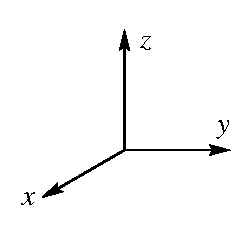
\includegraphics[scale=0.6]{figure/repere_orbitale.eps} & 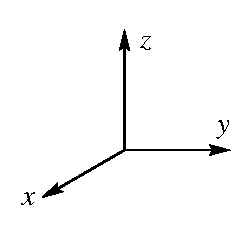
\includegraphics[scale=0.6]{figure/repere_orbitale.eps} & 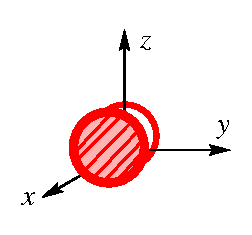
\includegraphics[scale=0.6]{figure/orbitale.eps} & 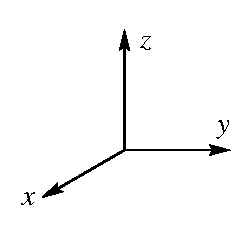
\includegraphics[scale=0.6]{figure/repere_orbitale.eps} & 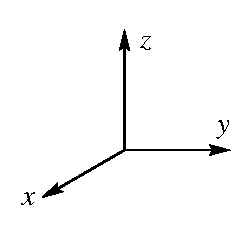
\includegraphics[scale=0.6]{figure/repere_orbitale.eps} \\
$1s$ & $2s$ & $2p_x$ & $2p_y$ & $2p_z$
\end{tabular}
\end{center}
%--------------------------------------------------------------------------
%\exo{\'Etude des \'el\'ements des 1$^\textrm{er}$ et 2$^\textrm{e}$ groupes}
%\begin{enumerate}[\bf 1)]
%\item Nommez les \'el\'ements alcalins.
%\item On donne la s\'erie des valeurs d'\'energies d'ionisation en kJ.mol$^{-1}$~: 375,6~; 402,9~; 418,7~; 495,7 et 520,1 pour ces \'el\'ements. Attribuez chaque valeur \`a un \'el\'ement, sachant qu'aucune valeur n'est donn\'ee pour le Francium. Expliquez la variation des \'energies d'ionisation dans la colonne.
%\item \'Ecrire la structure \'electronique \underline{de valence} des \'el\'ements du 2$^\textrm{e}$ groupe.
%\item Dites comment \'evoluent les grandeurs suivantes par rapport aux \'el\'ements alcalins~:
%\begin{enumerate}%[~~~-]
%\item degr\'e d'oxydation le plus souvent rencontr\'e,
%\item dimension,
%\item \'energie de premi\`ere ionisation.
%\end{enumerate}
%\end{enumerate}
%--------------------------------------------------------------------------
\exo{Configuration \'electronique et classification p\'eriodique}
\begin{enumerate}[\bf 1)]
\item Soit l'\'el\'ement $_{31}^{69}$Ga. \'Ecrire sa configuration \'electronique atomique.
Dans quel bloc de la classification p\'eriodique se trouve cet \'el\'ement~?
Sur quelle p\'eriode~?
Dans quelle colonne~?
\item M\^emes questions pour les \'el\'ements $_{~6}^{12}$C, $_{15}^{31}$P, $_{20}^{40}$Ca, 
$_{22}^{48}$Ti, $_{32}^{71}$Ge et $_{38}^{88}$Sr.
\item Comparez les rayons atomiques des \'el\'ements appartenant \`a une m\^eme p\'eriode/\`a une m\^eme colonne.
\end{enumerate}
\exo{Propri\'et\'es des \'el\'ements et classification p\'eriodique}
\begin{enumerate}[\bf 1)]
%\item \'Ecrire la structure \'electronique des ions suivants : I$^-$, Fe$^{2+}$, Cr$^{3+}$.
\item Classez les \'el\'ements suivants par ordre croissant de leur rayon atomique, puis par ordre croissant
de leur énergie de première ionisation :
\begin{enumerate}%[~~~-]
\item Rb, Li, Na, K
\item Cl, Na, P, S, Mg, Si, Al
\end{enumerate}
\item Commentez la variation de l'\'electron\'egativit\'e dans le tableau p\'eriodique. Classez les \'el\'ements suivants par ordre d\'ecroissant d'\'electron\'egativit\'e : K, F, Na, Cl, I.
\item Dites comment \'evoluent les grandeurs suivantes pour les alcalino terreux~:
\begin{enumerate}%[~~~-]
%\item degr\'e d'oxydation le plus souvent rencontr\'e,
\item rayon atomique,
\item \'energie de premi\`ere ionisation.
\end{enumerate}
\end{enumerate}
%
